\chapter{Evaluation}
\label{sec:part1-evaluation}

Thus far, we have described
  how we have applied
  the thesis of this dissertation---%
  that compiler backends
  should be generated
  from formal models of hardware---%
  in the realm of deep learning accelerators.
We first described the difficulties
  in developing compilers
  for deep learning accelerators.
We then described how these difficulties
  motivated the creation of
  3LA: a mostly-automated, end-to-end
  methodology
  for accelerator development.
(Note again that 3LA itself
  is not a contribution of this dissertation.)
We identified a specific problem
  within this domain
  as a problem of interest:
  mapping applications to accelerators.
To address this problem,
  this dissertation
  introduced
  \g,
  a tensor language
  which enables powerful rewriting techniques.
We then integrated \g 
  

This evaluation specifically evaluates
  \g's contribution
  to 3LA
  and to the thesis of this dissertation.
\cref{thesis:optimizations}
\cref{thesis:devtime}
\cref{thesis:correctness}
\hl{todo}

\hl{todo: direct evaluation vs indirect? that is, some of the eval is evaluating non-glenside things, but those things were enabled by glenside. we'd like to include them, because they do help prove the thesis, i.e. the testing results improve correctness. how to be explicit about what's evaluating glenside and what's not}
  

\hl{old:}

In this section, 
  we evaluate our prototype 
  %to evaluate 
  for end-to-end testing with \AppNum applications and three accelerator designs. We focus especially on
  %As part of this we also evaluate 
\begin{inlinelist}
\item automated identification of acceleration opportunities, and 
\item application-level validation using automated co-simulation.   
\end{inlinelist}
%
%\hl{Without the {\TLA} methodology, similar evaluation would require developing extensive bespoke compiler and simulation infrastructure, perhaps via BYOC. 
%We demonstrate that efficient end-to-end evaluation can be facilitated by a modular, extensible workflow with reusable components.}
Note that other tools provide very little automated support (if any)
%no existing automated methodology or tool addresses 
for these two capabilities, thus precluding any head-to-head comparisons. 
%Additionally, the prototype is focused on enabling testing,
  %rather than optimization,
% not intended to be
%   an optimizing compiler,
  %so we do not evaluate the performance
  %of the generated code.
%Besides the two focuses, we 
We also report on operator-level evaluation (accuracy and performance) and FPGA-based deployment.
%Further, {\TLA} is not intended to be a full-fledged compiler, and thus is not being evaluated in the performance of the compiled code or against other compilers.



\section{Target Accelerators}
\label{sec.eval-acc}

\hl{EVERYTHING BELOW THIS LINE IS STILL COPY-PASTE FROM 3LA}

We added support for three DL accelerators that provide hardware operators at different levels of granularity:
\begin{enumerate}[leftmargin=*]

\item \textbf{FlexASR} is an accelerator for speech and natural language processing (NLP) tasks that supports various RNNs~\cite{tambe20219}.
%
It uses a custom numeric data type called \textit{AdaptivFloat} for boosting the accuracy of quantized computations~\cite{tambe2020algorithm}.
%
% \hl{Our prototype supports FlexASR's linear layer and LSTM operations [@Gus/Mike, should we discuss how the LSTM pattern matching is handled? Perhaps give a footnote?].}
%
% FlexASR receives MMIO load and store commands from the host processor through an AXI interface. 
%
% These AXI commands have 128-bit data for various configurations, control, and memory operations. 

% FlexASR supports a variety of computations common in NLP applications, including various types of RNNs (e.g., Vanilla RNN, GRU, LSTM), fully connected layers, layer reduction (e.g., max and mean pooling), layer normalization, and the attention mechanism. 

\item \textbf{HLSCNN} is an accelerator optimized for 2D convolutions~\cite{whatmough201916nm}.
%
% It provides programmable support for arbitrary batch sizes, input and filter dimensions, and strides. 
%
%HLSCNN is designed to operate on mixed 8/16-bit fixed point data 
It operates on mixed 8/16-bit fixed point data
(8 bits for storing weights and 16 bits for computations).
%, and the feature map tensors are expressed in the NHWC layout format for providing better performance through parallelization.
%
% \hl{Our prototype compiler rewrites non-grouped 2D convolutions of appropriate sizes to HLSCNN's convolution operation.}

\item \textbf{VTA} is a parameterizable accelerator for tensor operations featuring a processor-like design~\cite{moreau2019hardware}.
%with an ISA and configurable parameters
%
It supports element-wise arithmetic operations as well as generalized matrix multiplication,
operating on 8-bit integer data.
%
% \hl{(Cribbed from CASES, please review/shorten.)}
% We chose VTA in part because TVM has special code generation support for VTA and also that unlike HLSCNN and FlexASR, which provide coarse-grained operations, VTA provides fine-grained instructions --- supporting VTA stresses the \textit{generality} of the {\TLA} methodology.
% As with other processor-like designs, the VTA ILA is based on its ISA~\cite{huang2018instruction}.
% In our prototype, as a proof of concept, we map matrix multiplication and bias addition to fixed sequences of VTA ILA instructions.
% In principle, it would be possible to implement a VTA ILA code generator more similar to TVM's built-in support for VTA (which produces VTA instructions to implement arbitrary TVM operators).

\end{enumerate}
%
%\hl{(Please review.)} 
% \recheck{@Yi: please review (combined LHS and RHS LoC and gave total for mappings).}
For each accelerator, we defined an ILA model and a set of \mapping rules.
%
The ILA models for FlexASR, HLSCNN, and VTA are approximately 5600, 1600, and 2100 lines of ILAng code (C++), respectively. 
%--- note that these ILAs serve the dual purposes of enabling compilation via the \TLA methodology as well as validating the RTL design.
%Note that 
The high-level synthesis (HLS) implementations
  of the accelerators are about 9300 (SystemC), 5100 (SystemC), and 6900 (Chisel) LoC, %lines of code, 
  respectively;
  the ILA specifications are thus of modest size,
  compared even to the relatively compact HLS implementations. 
%
For each \mapping rule, we represent the compiler side in Glenside IR, and the accelerator side %(via a wrapper API) 
as a program composed of ILA instructions (in a Python-embedded DSL). 
%\recheck{What's this wrapper API? Is it not in the python-embedded DSL?}
The total size of mapping rules (both the compiler and accelerator sides) for FlexASR (5 mappings), HLSCNN (1 mapping), and VTA (1 mapping) was 186, 22, and 49 LoC, respectively.
Recall that these mappings are polymorphic over tensor size on both sides, leading to general and compact representations. 
% **Aarti's original version: **
% \re{The ILA models do not include the \mapping rules. 
% For mappings, the LHS is represented in Glenside IR, and  the RHS is represented (via a wrapper API) as a program composed of ILA instructions (in a python-embedded DSL). Recall that these mappings are polymorphic over tensor size on both sides, leading to general and compact representations. 
% For FlexASR, we used 5 mappings (totalling 119 LoC on LHS, 67 LoC on RHS); for HLSCNN, we used 1 mapping (12 LoC on LHS, 10 LoC on RHS); for VTA, we used 1 mapping (38 LoC on LHS, 11 LoC on RHS). 
% }
Additionally, the BYOC-based code generators and runtimes for these accelerators are approximately 450, 300, and 900 LoC of C++, %\recheck{/Python},
%lines of code, 
respectively. 
%\recheck{@Yi, would it be more accurate to include the LoC for the Python codegens here also?}
%\recheck{It might also be more confusing/TMI since we didn't say much about their diffs and roles.}
%\recheck{Based on previous discussion, we agreed that we just LoCs for the mappings, which is added before, for counting the manual effort for providing the mappings. I think we should avoid adding more implementation details such as "API wrapper" or "python" stuff here.}
These indicate the implementation of the code generation module in our prototype, as well as reusable utilities for data movement, handling custom numerics, and emitting the low-level MMIO code for each selected accelerator offload for end-to-end simulation of the application.

\iffalse
%(Note that the SystemC HLS models are more difficult to simulate compared to using ILAng.
Note that simulating the SystemC HLS models requires extra effort and is less efficient compared to using ILAng.
  %do not provide the simulation capabilities provided by the ILAng-generated simulators. 
First, the ILA matches the MMIO interface while the SystemC model requires a custom driver. 
Second, the ILA model targets 
  the highest (architecture) level of abstraction,
%the highest level of abstraction by focusing on updates of the architecture state variables, 
  whereas general SystemC models may reflect low-level design details and are slower to simulate.
  \fi
%
%Additionally, the BYOC-based code generators and runtimes for these devices are approximately 450, 300, and 900 LoC of C++,
%lines of code, 
%respectively.
%
%Please see Appendix~\ref{app.operations} for a complete list of supported operations for the three accelerators.

\subsection{Target Applications}
\label{sec.eval-app}

% The MLPerf inference benchmark~\cite{mlperf,reddi2020mlperf} is a standardized collection of machine learning inference workloads, developed by more than 200 ML researchers and engineers across academia and industry.
% For our evaluation, we select models from the MLPerf inference benchmark so as to show our methodology's utility on state-of-the-art, industry-accepted workloads.
% Note that we do not run a true MLPerf benchmarking session, which involves connecting to the benchmark's custom-built test harness.
% Rather, we perform our own evaluation and gather our own metrics.

% \hl{most of the networks below are not actually part of mlperf inference...-GS}


%For the case studies, we considered the below applications which are developed by different teams and programmed in different DSLs:
%For our evaluation experiments, 
We considered \AppNum DL applications corresponding to common neural network models for language and vision tasks that contain operators supported by the three target accelerators.
%Many of these models loosely correspond to those included in the MLPerf benchmark~\cite{mlperf,reddi2020mlperf}, though 
We selected applications with reasonable size for human inspection and in-depth analysis.
% We generally chose relatively small models to reduce simulation times and simplify development. 
%ResMLP was chosen as a recent model that comprised primarily of linear layers and hence would be simple to support on VTA and FlexASR, while the LSTM word language model was chosen for its simplicity and correspondence to FlexASR's LSTM instruction.
%
% \hl{Let's give our reason for selection with each model --- the hl command does not play well with enumerations.}
%
\begin{enumerate}[leftmargin=*]

%\item \textbf{BERT} is a language representation model, for NLP tasks, that utilizes transformers with variable number of encoder layers and self-attention heads~\cite{devlin2018bert}.

\item \textbf{EfficientNet} is a recent convolutional neural network (CNN) designed for image classification~\cite{tan2019efficientnet}. 
%that uniformly scales network width, depth, and resolution~\cite{tan2019efficientnet}. 
% We chose it because it contains convolutions that could be accelerated by VTA and HLSCNN.
It has convolutions that are supported by VTA and HLSCNN.
% We chose EfficientNet as a recent CNN and hence a model likely to contain convolutions that could be accelerated by EfficientNet or VTA.

%\item \textbf{GNMT} is a neural network designed for language translation~\cite{wu2016google}.
%At its core, GNMT is powered by a deep chain of LSTM layers.

%\item \textbf{LSTM-S2T} is a speech recognition application designed based on the previously proposed LSTM recurrent neural network architecture~\cite{graves2014towards,tambe20219}. 

\item \textbf{LSTM-WLM} is a text generation application~\cite{pt2020wlm} implemented using an LSTM recurrent neural network architecture~\cite{graves2014towards}. The LSTM layer in this model is supported by FlexASR.
% It is given as an example in PyTorch's official example repository~\cite{pt2020wlm}.
% We chose this model because it contains an LSTM layer that could be accelerated by FlexASR.
%As detailed in Appendix~\ref{app.models}, 

% \yl{Current codegen has already supported retrieving hidden state and cell state}
% Note that we removed the unused final hidden and cell state return values so that the custom runtime deals only with a single output.
%simplifying the custom runtime's development
%by only dealing with a single output.
%to keep this application with a single output and to simplify the custom runtime development.
%Note that we made a small modification to this model in order to simplify the design of our BYOC-based code generator; namely, to avoid having to deal with multiple outputs, we eliminated the final hidden and cell state return values (which were not needed in this application).
%We made a small modification to the model after importing into Relay to match the semantics of our FlexASR LSTM code generator, namely by not returning the final hidden and cell states (unused in this application).
% We chose this model due to its simplicity and the fact its main computation could be accelerated by FlexASR's LSTM layer.

\item \textbf{MobileNet-V2} is a common CNN designed for mobile applications~\cite{howard2017mobilenets, sandler2019mobilenetv2}. We chose MobileNet-V2 due to its wide use, especially on embedded devices.
% \item \textbf{MobileNet-V2} is a common CNN designed for mobile and embedded vision applications that uses depth-wise separable convolutions~\cite{howard2017mobilenets, sandler2019mobilenetv2}. We chose MobileNet due to its wide use, especially on embedded devices. %  \hl{and in 8-bit quantized settings (corresponding to VTA's 8-bit hardware)}~\cite{jacob2017quantization}.

\item \textbf{ResMLP} is a recent residual network for image classification, comprised only of multi-layer perceptrons ~\cite{touvron2021resmlp}. Its linear layers could be accelerated by VTA and FlexASR.
% We chose ResMLP for its preponderance of linear layers that could be accelerated by VTA and FlexASR (despite not being a language model).

% \item \textbf{ResMLP} is a recent residual network, designed for image classification, comprised only of multi-layer perceptrons and no convolutional layers~\cite{touvron2021resmlp}.
% We chose ResMLP for its preponderance of linear layers that could be accelerated by VTA and FlexASR (despite not being a language model).

\item \textbf{Transformer} is an NLP model comprised primarily of attention mechanisms~\cite{vaswani2017attention}. 
% which outperformed earlier models that featured more complex recurrent cell structures~\cite{vaswani2017attention}.
We chose Transformer as a representative of recent popular NLP models. 
% which FlexASR is specialized for. <- unfortunately, it was not designed for them

\item \textbf{ResNet} is a popular CNN designed for image classification~\cite{he2016deep}. 
Besides ResNet-20, which we use in most of the evaluation, in \S\ref{sec.compilation-stats}, we additionally compare various implementations of ResNet-50 from MLPerf~\cite{mlperf} for its availability of different reference implementations.
%We use ResNet-20 for our end-to-end testing because its small size reduces simulation times; in \S\ref{sec.compilation-stats} we use ResNet-50 for comparing multiple different implementations because of the easy availability of its reference implementations.


%\item \textbf{Q-MobileNet} is a quantized variant of the MobileNet neural network~\cite{howard2017mobilenets}.

\end{enumerate}
%
% With the exception of the minor change for LSTM-WLM's unused outputs, 
All applications were mapped to accelerators \emph{without any manual modifications}.
%\hl{(Decide if the appendix is necessary.)} 
%Detailed parameters for these applications are given in Appendix~\ref{app.models}.
\begin{table*}
  \centering
  \caption{
  \textbf{End-to-end compilation statistics.}
  %\hl{TODO: add "total" column on RHS}
  The total number of Relay operators (row 3) is given as a proxy
  for program complexity.
  In rows 4-6, we include rewrites for only one accelerator at a time; we do not offload to multiple accelerators at once like in \S\ref{sec.end-to-end}. Flexible matching identifies significantly more offloads than exact matching.
  Abbreviations: MN: MobileNet, Trans.: Transformer, and TF: TensorFlow.
  }
  \label{tab.compilation}
  %\begin{small}
  \resizebox{\textwidth}{!}{
  \begin{tabular}{|clrrrrrr||rrr|}
  \hline
  \multicolumn{11}{|c|}{Application Statistics} \\ \hline
  \multicolumn{1}{|c|}{1} &
    \multicolumn{1}{|l|}{Application} &
    \multicolumn{1}{c|}{EfficientNet} &
    \multicolumn{1}{c|}{LSTM-WLM} &
    \multicolumn{1}{c|}{MN-V2} &
    \multicolumn{1}{c|}{ResMLP} &
    \multicolumn{1}{c|}{Trans.} &
    \multicolumn{1}{c||}{ResNet-20} &
    \multicolumn{3}{c|}{ResNet-50}
    \\ \hline
  \multicolumn{1}{|c|}{2} &
    \multicolumn{1}{|l|}{Source DSL} &
    \multicolumn{1}{c|}{MxNet} &
    \multicolumn{1}{c|}{PyTorch} &
    \multicolumn{1}{c|}{PyTorch} &
    \multicolumn{1}{c|}{PyTorch} &
    \multicolumn{1}{c|}{PyTorch} & 
    \multicolumn{1}{c||}{MxNet} &
    \multicolumn{1}{c|}{PyTorch} &
    \multicolumn{1}{c|}{ONNX} &
    \multicolumn{1}{c|}{TF}
    \\ \hline
  \multicolumn{1}{|c|}{3} &
    \multicolumn{1}{|c|}{\#Relay Ops} &
    \multicolumn{1}{c|}{232} &
    \multicolumn{1}{c|}{578} &
    \multicolumn{1}{c|}{757} &
    \multicolumn{1}{c|}{343} &
    \multicolumn{1}{c|}{872} &
    \multicolumn{1}{c||}{494} &
    \multicolumn{1}{c|}{709} &
    \multicolumn{1}{c|}{194} &
    \multicolumn{1}{c|}{609}
    \\ \hline \hline
  \multicolumn{11}{|c|}{Number of Static Accelerator Offloads Identified Using Exact Matching/Flexible Matching} \\ \hline
  \multicolumn{1}{|c|}{4} &
    \multicolumn{1}{|l|}{FlexASR} &
    \multicolumn{1}{r|}{0/35} &
    \multicolumn{1}{r|}{1/1} &
    % This is 1 if we manually rewrite add -> bias_add.
    \multicolumn{1}{r|}{0/41} &
    \multicolumn{1}{r|}{0/38} &
    \multicolumn{1}{r|}{0/66} &
    \multicolumn{1}{r||}{2/22} &
    \multicolumn{1}{r|}{0/54} &
    \multicolumn{1}{r|}{0/54} &
    \multicolumn{1}{r|}{0/54}
    \\ \hline 
  \multicolumn{1}{|c|}{5} &
    \multicolumn{1}{|l|}{HLSCNN} &
    \multicolumn{1}{r|}{35/35} &
    \multicolumn{1}{r|}{0/0} &
    \multicolumn{1}{r|}{40/40} &
    \multicolumn{1}{r|}{0/0} &
    \multicolumn{1}{r|}{0/0} &
    \multicolumn{1}{r||}{21/21} &
    \multicolumn{1}{r|}{53/53} &
    \multicolumn{1}{r|}{53/53} &
    \multicolumn{1}{r|}{0/53}
    \\ \hline 
  \multicolumn{1}{|c|}{6} &
    \multicolumn{1}{|l|}{VTA} &
    \multicolumn{1}{r|}{0/35} &
    \multicolumn{1}{r|}{36/36} &
    \multicolumn{1}{r|}{1/41} &
    \multicolumn{1}{r|}{38/38} &
    \multicolumn{1}{r|}{66/66} &
    \multicolumn{1}{r||}{0/22} &
    \multicolumn{1}{r|}{0/24} &
    \multicolumn{1}{r|}{0/24} &
    \multicolumn{1}{r|}{0/24}
    \\ \hline % \hline
\iffalse
  \multicolumn{8}{|c|}{Number of Static Accelerator Invocations using Flexible Matching} \\ \hline
  \multicolumn{1}{|c|}{7} &
    \multicolumn{1}{|l|}{FlexASR} &
    \multicolumn{1}{r|}{0} &
    \multicolumn{1}{r|}{1} &
    \multicolumn{1}{r|}{2} &
    \multicolumn{1}{r|}{26} &
    \multicolumn{1}{r|}{2} &
    \multicolumn{1}{r|}{-} 
    \\ \hline 
  \multicolumn{1}{|c|}{8} &
    \multicolumn{1}{|l|}{HLSCNN} &
    \multicolumn{1}{r|}{35} &
    \multicolumn{1}{r|}{0} &
    \multicolumn{1}{r|}{40} &
    \multicolumn{1}{r|}{0} &
    \multicolumn{1}{r|}{21} &
    \multicolumn{1}{r|}{-}
    \\ \hline 
  \multicolumn{1}{|c|}{9} &
    \multicolumn{1}{|l|}{VTA} &
    \multicolumn{1}{r|}{35} &
    \multicolumn{1}{r|}{36} &
    \multicolumn{1}{r|}{41} &
    \multicolumn{1}{r|}{38} &
    \multicolumn{1}{r|}{22} &
    \multicolumn{1}{r|}{-}
    \\ \hline 
\fi
  \end{tabular}
  }
  %\end{small}
  \end{table*}
\subsection{Identifying Acceleration Opportunities}
\label{sec.compilation-stats}

%We examined \TLA's capabilities in identifying acceleration opportunities. % using our compiler prototype.
%
We took the \AppNum DL applications, developed by different teams in different DSLs, and compiled them for the three target accelerators.
% down to \hl{a synthetic processing platform that contains a host processor and the three target accelerators}.
%
% Without any manual accelerator-specific program restructuring and modification, 
Our compiler successfully generated code that exploits the accelerators for supported computations.
%
%Furthermore, we demonstrate full-system deployment, running \TLA-generated code on physical hardware through FPGA emulation.

%\subsubsection{Portability and Flexible Matching}

Table~\ref{tab.compilation} shows the compilation statistics of using exact matching and flexible matching.
%
%It describes 
  %the application source language (Row~2) 
  %and 
  %the program complexity using the number of Relay operators as a proxy (Row~3). 
%
%It reports the number of identified accelerated operations in FlexASR, HLSCNN, and VTA when using exact/flexible matching in Rows~4-6. 
%
Note that some accelerator operators correspond to multiple Relay operators; in particular, 
%the 35-step FlexASR LSTM in LSTM-WLM is 566 operators 
the LSTM RNN in LSTM-WLM corresponds to 566 Relay operators 
and maps to \textit{one} FlexASR operator, which shows \TLA effectively overcoming a dramatic granularity mismatch between the compiler IR and accelerator operators.
%
%It also reports the corresponding statistics for using flexible matching in Rows~7-9.
%
%\hl{Computations in A, B, and C can be offloaded to accelerator X and Y.}
%
% \hl{Further, With flexible matching, the compiler optimizes D, E, and F by identifying and offloading to Z.}
%
%\hl{With no accelerator-specific modification on the programs}, 

Our results demonstrate \TLA's viability across a range of DL applications and accelerators with the successful identification of acceleration opportunities
%
%Furthermore, it provides 
and provide
evidence for the utility of flexible matching. % is useful for optimization.
%
% This demonstrates portability with the successful exploitation of accelerators without accelerator-specific modification and provides evidence that flexible matching is useful for optimization.
%
%For example, flexible matching revealed several offloads to FlexASR's linear layer in MobileNet-V2 by rewriting \texttt{add} to \texttt{nn.bias_add} (a special case of adding a vector to a tensor) when the dimensions were appropriate.
%\hl{Gus is rewriting this sentence.}
%\hl{AG: please relate text to entries/numbers in table, and add contrast with numbers for exact matching.}
%For example, flexible matching uncovered 41 offloads to FlexASR's linear layer in MobileNet-V2 by rewriting \texttt{nn.dense} to \texttt{nn.dense} followed by an add of a zero tensor.
%
For example, the linear layer rewrite %described in 
(\S\ref{sec.method.flexible})
  resulted in 66 invocations of FlexASR's linear layer
  in Transformer and 38 in ResMLP, in comparison to exact matching that produced no match. 
%Also note that 
Furthermore, certain Glenside rewrites~\cite{smith2021pure} that implement the \texttt{im2col} optimization~\cite{chellapilla2006high} 
rewrite 2D convolutions into matrix multiplications;
for VTA, this resulted in \emph{additional} 35 invocations in EfficientNet, 22 in ResNet-20, and 40 in MobileNet-V2.
Hence, flexible matching allowed us to support 2D convolutions on VTA even when 
there is no \mapping that maps 2D convolutions to VTA instructions.
%the prototype code generator did not explicitly implements 2D convolutions via VTA instructions.
%, despite the fact the prototype code generator did not explicitly implement 2D convolutions via VTA instructions.
Another rewrite
  that turns lone matrix multiplications
  into linear layers
  (by a zero-vector bias)
  works in concert with the \texttt{im2col} rewrites,
  resulting in offloads of 2D convolutions
  onto FlexASR  
  in EfficientNet, MobileNet-V2, and ResNet-20---%
  thus allowing an accelerator for NLP applications
  to also accelerate vision applications.
%result in many more offloads to VTA in that table; this is due to 2D convolutions being rewritten into matrix multiplications
%
Note that these additional acceleration opportunities
  were identified automatically
  and are examples of \textit{emergent effects} resulting from simple, reusable (accelerator-agnostic) compiler IR rewrite rules.

We additionally
  evaluate the robustness
  of flexible matching
  by comparing
%To demonstrate flexible matching robustness,
  %we used 
  the three implementations of ResNet-50
  from MLPerf~\cite{reddi2020mlperf}
  %giving the results 
  in Table~\ref{tab.compilation}, right.
Their Relay representations 
  differed in subtle ways (such as in reshaping operators)%
  \footnote{
For example, the TensorFlow implementation
  takes data in NHWC format rather than NCHW;
  Glenside can rewrite convolutions to use NCHW.}
  and are reflected in the difference in results of exact matching.
%The results highlight the robustness of flexible matching, 
Flexible matching found the same (increased) number of matches for each accelerator, regardless of its source DSL.

% We additionally assessed 
%   the ability of flexible matching to accommodate
%   differences between multiple real-world implementations 
%   %(which we term ``robustness'') 
%   of the same model,
%   %by analyzing the results 
%   %of applying flexible matching 
%   %to multiple implementations of the same model, 
%   all in different DSLs.
% Namely, we used the three implementations of ResNet-50
%   from the MLPerf benchmark~\cite{reddi2019mlperf},
%   %in PyTorch, ONNX, and TensorFlow
%   %and applied flexible matching
%   %after importing them into TVM,
%   giving the results in the right half of Table~\ref{tab.compilation}.
% The Relay representations of these models
%   differed in subtle ways (such as in reshaping operators), as indicated by the different numbers of operators in Row 3.
% In particular,
%   the TensorFlow implementation
%   takes data in NHWC format rather than NCHW,
%   which is the version used by the other implementations
%   and our exact matcher;
%   Glenside was able to rewrite its convolutions to use NCHW format,
%   thereby finding additional matches.   
% The results highlight the robustness of flexible matching, which was able to find the same increased number of matches for each accelerator, independent of the source.
% %However, when we applied flexible matching,
%   %there were fewer differences (give numbers of matches).
% %This suggests that the rewrite rules in Glenside
%   %were able to convert these different but equivalent implementations
%   %of the same model
%   %into a single representation,
%   %relieving developers of the burden of
%   %manually reconciling such differences.
% %SM Alternate text assuming results added to table 1: The results for ResNet-50 highlight the robustness of flexible matching - even with three different implementations of the model from different sources and subtle differences in their corresponding Relay representation, flexible matching was able to find the same number of matches independent of the source for each accelerator. }


% We utilized the Xilinx SDK~\cite{xsdk} to pass the accelerator instructions (i.e., MMIO commands) to the FPGA for invoking the accelerator interface and ultimately running LSTM and linear layer workloads onto the hardware. 
% The accelerator results read from the FPGA hardware exactly matched the ILA simulation -- confirming bit-level correctness of the {\TLA} methodology on a commodity hardware platform. 
% This also proves that we can rely on the ILA simulation-based approach for fast verification velocity after hardware ECOs rather than performing FPGA emulation which imposes significant engineering effort overheads. 
% \hl{Which application was this with the linear layer workload - need to mention that. Also why just this one application. Need to explain that.}


\subsection{Per-Operator Evaluation}

% We have performed simulation-based validation to check the correctness of all the compiler IR to accelerator mappings for our target accelerators, with verification tasks of the VT1, VT2 and VT3 in Figure \ref{fig.mapping}. 
% During the simulation, the models from two sides of the mapping are given the same input tensor data, and we measure the relative errors between the results from two sides. 

% 1. what we are checking
% 2. describe the results in the table
% 3. what do the results tell us

%Although comparing the accuracy of individual operators
Although evaluating individual operators
  does not suffice to characterize
  how an accelerator performs on a full application,
  it is a basic first step
  and provides 
  insights on the identified acceleration opportunities.
  %validation of 
  %the given compiler IR--accelerator mappings.
  %it provides (i) a basic first step toward end-to-end
  %testing and (ii) validation
  %of the given compiler IR-accelerator mappings.
%Due to auto-generated ILA simulators, this 
  % is readily enabled by the {\TLA} methodology.
%The auto-generated ILA simulators
  % readily enable this in the {\TLA} methodology.
Here, we discuss both functional validation and performance evaluation at the operator level.

%Modern accelerators often adopt custom numerics for achieving better power-performance efficiency.
%
%For example, in our cases, FlexASR and HLSCNN use the AdaptivFloat and 8/16-bit fixed point data types, respectively.
%
%This means checking the IR-accelerator mappings must account for the numerical differences.
%
%%To separate the effect of numerics and focus on the definition of operations, we use abstract data types to formally verify the equivalence
%(demonstrated through a proof-of-concept case study).
%
%On the other hand, 
%%In addition, to precisely capture the numerical differences, we use simulation to compare accelerator executions (using an ILA simulator) against the IR semantics (using an IR interpreter).

%\para{Simulation-Based Validation}

% Recognize the deviation due to custom numerics.
% How: the setup
% Summarize: op-level accuracy is relatively good

% Among the three verification tasks, we see negligible mismatch in VT1, which is from the rounding errors of floating-point numerics. 
% In VT3, we have an exact match between accelerator ILA and accelerator implementation simulation results, despite the modeled accelerator implementations may have their customized numerical representation (e.g., customized 8-bit floating point system in FlexASR \cite{tambe2020algorithm} and 8-bit fixed point representation in HLSCNN). 
% This is because the generated simulator from accelerator ILA supports custom numeric computation from the accelerators' original implementation as "plug-ins" to fully model the behaviors of the accelerator in both computation definition and numerical representation.
% Based on VT1 and VT3, we can check the mapping correctness by performing VT2. 

\subsubsection{Functional Validation}

\begin{table}
\caption{
\textbf{
Simulation-based validation results for checking {\mapping}s.
}
% We measure the relative errors of VT2 using tensors' Frobenius Norm as:
% $Error = \norm{Out_{ref} - Out_{acc}}_F / \norm{Out_{ref}}_F$. 
% We measure the relative errors of the accelerator program fragment simulation results against the compiler simulation results on host processor with the following function using tensors' Frobenius Norm:
% $Error = \frac{\norm{Out_{ref} - Out_{acc}}_F}{\norm{Out_{ref}}_F} * 100\%$. 
The average relative error (Avg. Err.) and the standard deviation (Std. Dev.) of errors are measured 
%for simulations 
over 100 test inputs. % with randomly generated inputs.
% See Table \hl{TODO} in the Appendix for the complete validation results of all IR-accelerator mappings.
For VTA, 
%we compared GEMM, add, and max operations; 
there was no error because the host supports 
8-bit integer operations.
%these operations in 8-bit integer.
}
\label{tab.layer-sim}
\centering
\begin{small}
\begin{tabular}{|c|l|l|r|r|}
\hline
  & Accel. & Operation & Avg.Err. & Std.Dev.  \\
  \hline \hline
  1 & VTA & All ops & 0.00\% & 0.00\% \\ % \hline
  2 & HLSCNN & Conv2D & 1.78\% & 0.16\% \\ % \hline
  3 & FlexASR & LinearLayer & 0.84\% & 0.29\% \\ % \hline
  4 & FlexASR & LSTM & 1.21\% & 0.19\% \\ % \hline 
  5 & FlexASR & LayerNorm & 0.27\% & 0.20\% \\ % \hline
  6 & FlexASR & MaxPool & 0.00\% & 0.0\% \\ % \hline
  7 & FlexASR & MeanPool & 1.79\% & 0.28\% \\ % \hline
  8 & FlexASR & Attention & 4.22\% & 0.09\% \\ 
\hline
\end{tabular}
\end{small}
\end{table}

The {\TLA} methodology readily enables operator-level validation through auto-generated ILA simulators.
%For operator-level testing,
%compiler IR-accelerator mappings through simulation, 
In our experiments, we 
%generated 100 random test inputs and 
compared the outputs of the accelerator ILA simulator and those of TVM's runtime on host.
%
The accelerator ILA simulators precisely model the data types used by the accelerators.
%
%\hl{Specifically, VTA, HLSCNN, and FlexASR use 8-bit integer, mixed 8/16-bit fixed point, and AdaptivFloat, respectively.}
%
%For the reference results (TVM's runtime), we use 8-bit integer, 32-bit floating point, and 32-bit floating point when checking VTA, HLSCNN, and FlexASR operations, respectively. These are the closest host processor data types to those used by the accelerators. 
For the reference results (TVM's runtime), we use 8-bit integer for comparing against VTA and 32-bit floating point for the other accelerators, as these are the closest host processor data types to those used by the accelerators. 
%
We measure the relative errors by using the standard Frobenius Norm~\cite{lapack} for the tensors based on the reference and accelerator generated output values as follows:
%$Error = \norm{Out_{ref} - Out_{acc}}_F / \norm{Out_{ref}}_F$.
$Error = \| Out_{ref} - Out_{acc} \|_F / \| Out_{ref} \|_F$.
\iffalse
\[
Error = \frac{\norm{Out_{ref} - Out_{acc}}_F}{\norm{Out_{ref}}_F} * 100\% 
\]
\fi
% Here, $Out_{ref}$ and $Out_{acc}$ are the IR reference and accelerator outputs, respectively.

We validated all types of operators supported by the target accelerators.
Table~\ref{tab.layer-sim} shows a representative subset of the validation results: four {\mapping}s (Rows~1-4) that are used in the full application compilation (Table~\ref{tab.compilation}) and four additional mappings for non-trivial operations (Rows~5-8).
%We omitted validation results of other mappings, e.g., for trivial operations \textit{add} and \textit{max}. \hl{SM: Are these the only results omitted?}
% See Table \hl{TODO} in the Appendix for complete validation results of all IR-accelerator mappings.
% Table~\ref{tab.layer-sim} shows the validation results. 
% The top four compiler IR-accelerator mappings are used in our end-to-end compilation experiments. 
% We also perform simulation validation for all the other mappings, but some of them are trivial operations, such as \textit{add} or \textit{max} in VTA operations. 
% Here we show four more non-trivial mappings' validation results.
%
%Columns~1 and~2 indicate the accelerator and the supported operation for each compiler IR-accelerator mapping, respectively.
%
%Columns~3 and~4 report the average relative error and the standard deviation, respectively, over the 100 test inputs.
%
Note that some mappings introduce no numerical differences; e.g., the TVM runtime supports 8-bit integer execution, so the results for VTA match perfectly.
%For mappings that are not affected by numerical differences, e.g., the VTA-supported GEMM, we see exact matches in the results.
%
For other mappings, we see deviations caused by the custom numerics, especially for complex operators such as the attention operator on FlexASR.  
% yes
%\hl{AG: comment on deviations? does this mean we should watch end-to-end more carefully?}
Such deviations should be carefully assessed
  in the context of application-level validation,
  as even small deviations could accumulate and affect the final accuracy.

% Table \ref{tab.layer-sim} shows the simulation results for compiler IR-accelerator mappings of the three different accelerators.
% The range and distribution of the testing inputs are determined based on the target application of the accelerators and the input values are quantized.
% VTA is using standard 8-bit integer datatype and shows an exact matched with the Relay IR program fragment results which also using the same 8-bit integer for computation. 
% However, since there is no support for the customized floating-point or fixed point numerics used in HLSCNN and FlexASR, the Relay IR program for these mappings simulated with standard 32-bit floating-point representation. 
% Among these mappings, we only observe small relative errors, which shows the correctness of the mappings with acceptable deviation with the custom numerical representation in the accelerators.

\subsubsection{Performance Evaluation}

%The {\TLA} methodology enables performance evaluation on the operators that will be accelerated in the full application compilation.
%--- allowing comparing the precise number of exact offloaded host operators against the invoked accelerator operators.
%In our experiments, we 
We also evaluated the performance gain of offloading operations from the host to accelerators 
%(identified as reported in Table~\ref{tab.compilation}) 
using cycle counts as the performance metric, since we did not have clock frequencies for an SoC containing the host and accelerators.
%\footnote{
%Precise performance modeling depends on various factors, e.g., processing technology node, that may not yet be available for prototype accelerators, like in HLSCNN and VTA.
%We chose cycle count as the appropriate metric for (micro-)architectural design evaluation.
%}
%\aarti{We used this metric since clock rates might vary and are, in fact, a design consideration.}
For accelerators, we derived the cycle counts based on their cycle-accurate models
(VTA's Chisel model
%TSIM for VTA
and FlexASR's and HLSCNN's SystemC models).
%RTL implementation (FlexASR and HLSCNN)
%\yl{Right now FlexASR and HLSCNN performance models are based on their cycle-accurate SystemC simulation model}
%or the cycle-accurate Chisel-generated simulator (VTA).
%We measured average cycle counts of operators executed in TVM's runtime on host (EPYC0000) over 2000 random inputs.
For the host, we measured averaged cycle counts (1000 random inputs) in TVM's runtime
%, averaging over 2000 random inputs 
on one pinned EPYC-7532 core.

% I don't think we need this for dissertation.
\begin{figure}
  \centering
  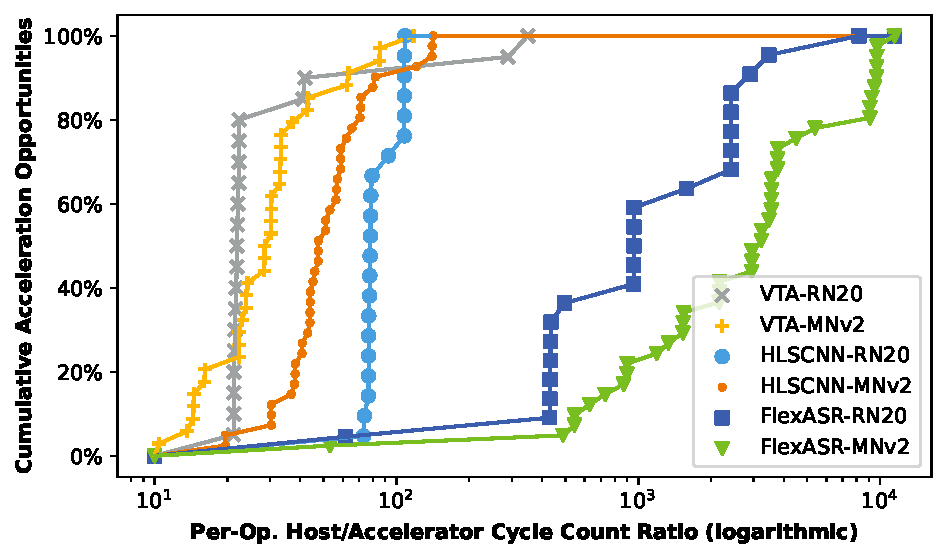
\includegraphics[width=.65\linewidth]{3la/Figures/performance.pdf}
  \caption{
\textbf{
Cumulative distribution of per-operator performance gains of all identified acceleration opportunities} in ResNet-20 (RN20) and MobileNet-V2 (MNv2) on the three accelerators.
%VTA, HLSCNN, and FlexASR.
Each point represents an operation offloaded from the host to the accelerator (as identified by flexible matching, Table~\ref{tab.compilation}).
The $x$-axis shows the host-to-accelerator cycle count ratio of each offloaded operation 
%(the bigger the better); 
and the $y$-axis shows the cumulative distribution of offloaded operations. Points and plots more to the right are better; e.g., coarse-grained operators, supported with higher parallelism in FlexASR, offer greater speedup compared to the fine-grained operators in VTA. %\sm{Change Accumulative in figure to Cumulative.}
%the y-axis accumulates toward all identified acceleration opportunities in an application.
%The measurement is done on 2000 random inputs from the CIFAR-10 dataset~\cite{cifar10}. \yl{The test inputs are not from CIFAR-10 dataset. It is just a random input with the same shape to the layer input in the applications}
}
  \label{fig.performance}
% \Description{}
\end{figure}

Fig.~\ref{fig.performance} shows the performance gains (ratio of host to accelerator cycles) of all identified acceleration opportunities in ResNet-20 and MobileNet-V2 when operations are offloaded from the host to VTA, HLSCNN, and FlexASR, respectively. 
%Figure~\ref{fig.performance} shows the cycle count ratios of all offloaded operations (from the host to the accelerator) in ResNet-20 and MobileNet-V2 when compiled to VTA, HLSCNN, and FlexASR.
%the three accelerators.
%Each point represents an operation offloaded from the host to the accelerator.
Overall, as expected, all offloads resulted in performance gains relative to the host; we also see that accelerators providing coarser-grained operators (e.g., FlexASR), supported with higher parallelism, achieve higher performance gain per operator compared to finer-grained accelerators like VTA. %\sslyu{Is this really something we should highlight? We don't discuss performance gains of coarse-grained vs fine-grained accelerators in the intro; our point is just that we gain performance compared to the host, which is what we're aiming for.}
%\aarti{
%Although the graph does not compare operator attributes, such as convolution strides, such per-operator performance evaluation can also provide additional insights on how these properties affect the performance of offloaded operators. 
%such as how the Conv2D operator performs under different stride attributes and \texttt{im2col} matrix dimensions.
%This could be useful in future work for performance optimization.
%} 
%\sslyu{Are we reporting any data to suggest that conclusion? We shouldn't say this if we don't. Otherwise, we could say that our methodology for getting the cycle counts could be used for assessing these issues.}
%We also find such per-operator performance evaluation insightful.
%Take VTA for example, {\TLA} provides a convenient way to analyze, within a real application, how the Conv2D operator performs under different convolution stride attributes and \texttt{im2col} matrix dimensions.
% From the operator-level performance analysis, we also see that VTA is not always good.
%We also found that the same Conv2D operator of VTA performs better when the convolution strides attributes align well with the \texttt{im2col} matrix dimensions---up to 10x difference in performance gain.
% \yl{VTA performs better stride attributes in the Conv2D are larger than 1. The reason is that larger strides would reduce the matrix size for matrix multiplications after doing im2col.}
%By measuring the performance of both running 2D Convolutions layers and running corresponding Dense matrix multiplications obtained from the \texttt{im2col} optimization, we found that VTA does not always gain performance from the optimization unless the strides attributes of the convolution layer keep the \texttt{im2col} matrix dimensions small enough. 
%(\yl{Not sure we should put the comparison between our codegen with original VTA codegen in here though. We are not using the original VTA codegen for Conv2D in our experiment. Also this comparison deviates a little from the other comparisons between acc. and host CPU.})
%(\mh{See numbers in the table and conv2d configurations of those layers}) 
%Under certain settings, the optimization brings up to 4x speed-up while in some other cases, it makes 2x worse performance compared with the baseline operator.
%Such per-operator performance evaluation provides insights on the identified acceleration opportunities in the full application compilation and is critical to more thorough performance optimization.
%It is critical to more thorough performance optimization.
%In this way, enabling per-operator performance evaluation would help accelerator users identify the right place to apply such optimizations.
%This study demonstrates that the {\TLA} methodology enables performance evaluation at the operator level, providing insights on how the identified acceleration opportunities perform in a full application.
%This is critical to future performance optimization.


\iffalse
\para{Proof-Based Formal Verification}
\label{sec:fv}
%%% there are differences, likely due to numerics, and we want to check that using abstract data types
%%% summrize: we can formally prove small scale op-level mappings

%%% As described earlier in Section~\ref{sec.method.verif}, verification of the full flow includes task VT2, which verifies equivalence of the ILA program fragment on the compiler side with that on the accelerator side. 
%%% This section describes a proof-of-concept study on the  Relay and FlexASR fragments for the temporal max-pooling application (see Appendix for the ILA code).

%%% In formally verifying the mappings, we use abstract data types to separate the effect of custom numerics.

The key challenges in formally verifying mappings between fragments that represent DL computations include:
\begin{inlinelist}
  \item handling nested loops, for both compiler side and accelerator side, that iterate through tensor elements, and
  \item relating tensor variables between the two sides which may employ various tiling mechanisms.%, and
%   \item handling custom numerics.
\end{inlinelist}
%
%%% Although the code of each ILA fragment is small, there are challenges due to:
%%% \begin{itemize}
%%%     \item multiple nested loops: 4 levels of nesting on Relay side, 3 on FlexASR side.
%%%     \item \emph{aligning} the nested loops for checking equivalence
%%%     \item mapping the input matrix to a special customized tiling provided by FlexASR~\cite{tambe20219}. \footnote{\hl{We ignore the FlexASR numerics accuracy in this study.}}
%%% \end{itemize} 
%
As a proof-of-concept study, we considered the Relay and FlexASR fragments for the FlexASR MaxPool IR-accelerator mapping. These fragments both have 
3+ nested loops, and the relation between the two fragments must account for a special customized tiling provided by 
FlexASR~\cite{tambe20219}.
For this study, we considered %
equivalence of the fragments over %
fixed-sized tensors with symbolic data,\footnote{Formally modeling custom numerics is left to future work.} and implemented verification using two methods:
\begin{inlinelist}
  \item bounded model checking (BMC)~\cite{biere2003bounded}, and 
  \item program verification using constrained Horn clauses (CHCs)~\cite{komuravelli2016smt}. 
\end{inlinelist}
%
The BMC-based method unrolls all the loops in both fragments, which is straightforward but may fail to scale for large-sized tensors.
%
The CHC-based method is given a product program of the two fragments and uses \emph{relational} loop invariants, i.e., formulas that relate the two fragments at intermediate loop boundaries (details are beyond the scope of this paper). 
%
This avoids loop unrolling and can handle large tensors. 
Both methods use Z3~\cite{de2008z3} as the underlying SMT solver.

% In our case study, we provided invariants that capture the customized tiling of FlexASR for fixed-sized matrices. 
% (In future work, we will consider automatic inference of such loop invariants.) 

While ILAng directly supports BMC, we manually created CHCs for the CHC-based method.
%for a 2D MaxPool operation in FlexASR. 
We also supplied the relational invariants that capture the customized tiling of FlexASR.
%
In future work, we plan to automate CHC generation, which will allow formal verification of other IR-accelerator mappings used in this paper.
%
Table~\ref{tab.verif-formal} shows the results for this case study for various dimensions of the 2D input matrix (Column~1), with runtimes of the BMC-based and CHC-based verification methods in Columns~2 and~3, respectively. 
%
The BMC-based method was able to verify equivalence of mappings with small-sized matrices, but timed out (with a 3-hour time limit) on the $16 \times 64$ matrix that was used for simulation-based validation. % (based on the available accelerator testcases).
%
In contrast, the CHC-based method was faster than BMC and successfully verified mappings with larger matrices. These results are encouraging and demonstrate how the \TLA methodology enables formal verification of key steps in the compilation flow. 
\fi
%
% Our results for both methods are reported in Table~\ref{tab.verif-formal}, for verification runtime on input matrices of various dimensions.
%TODO: add interpretation

%\subsection{End-to-End Testing}
\subsection{Application-Level Validation Through Co-Simulation}
\label{sec.end-to-end}

%Having validated the IR-accelerator mappings, we 
%We next explore how the small numerical differences at the level of individual operators affect the results of evaluating full applications.
%One main goal of the {\TLA} methodology is to
  %allows us to 
  %explore this through 
We performed application-level co-simulation
  %namely 
  by using the
  ILAng-generated simulators for accelerator computations
  and the host CPU for the rest of the computation.
%want to check if minor deviations at the single operation level will influence application-level behavior.
%
%Therefore, we performed application-level co-simulation on several applications which offload various computations to FlexASR and HLSCNN, the two accelerators that utilize custom numerics. (By co-simulation we mean simulating the software running on the host processor along with the operations off-loaded on the accelerator using the ILA simulator.)
%
%Specifically, we examined models that we were able to train and deploy on \hl{all of the devices (SM: unclear)} supported in our prototype:
We considered three applications,
  which between them provide opportunities to use
  each of the three accelerators: %,
  %as well as even combinations of them:
\begin{inlinelist}
  \item LSTM-WLM, where we accelerate linear layer and LSTM operations on FlexASR;
  \item ResNet-20, where we accelerate convolutions on HLSCNN and linear layers on FlexASR; and
  \item MobileNet-V2, where we accelerate convolutions and linear layers as in ResNet-20 and additionally accelerate both these operations on VTA (due to the \texttt{im2col} rewrites).
\end{inlinelist}
In ResNet-20 and MobileNet-V2,
  we were able to
  \emph{explore using HLSCNN and FlexASR together and separately}, simply by varying which 
  %IR-accelerator rewrites 
  {\mapping}s
  we included in flexible matching.

%Each of the three accelerators considered is used in some application, and even combinations of these accelerators are used in individual applications:
%\begin{inlinelist}
  %\item LSTM-WLM, whose linear layer and LSTM operations are supported by FlexASR;
  %\item \hl{ResMLP, whose linear layers are also supported by VTA}; and
  %\item ResNet-20 and MobileNet-V2, whose convolutions are supported by HLSCNN and whose linear layers are also supported by FlexASR, \emph{allowing us to explore using the accelerators together and separately}, simply by varying which IR-accelerator rewrites we include in the flexible matching step.
%\end{inlinelist}
%LSTM-WLM, which offload to FlexASR the LSTM layer and linear layer operations, respectively.
%
%We also considered MobileNet and ResNet, which both offload 2D convolution and linear layer operations to HLSCNN and FlexASR, respectively.
%
%(We compiled to two target accelerators by including the IR-accelerator rewrite rules for both accelerators.)
%
% As a sanity check \hl{(Was it a sanity check? It seems like an interesting case in its own right. -- Safety net in case we don't have a fully-matched VTA e2e in time so that we can drop it.)}, we also evaluated a quantized MobileNet on VTA, comparing application results under \hl{integer numerics, which have no rounding error}.


% Although the IR-accelerator mappings simulation shows acceptable relative errors, we don't know the mapping errors on a specific trained model or how these errors will accumulate across the layers and more importantly, how the numerical difference of the outputs will hurt the application-level results, such as the inference accuracy. Therefore, it is important to perform an application-level co-simulation to measure the correctness of the program running on the heterogeneous platform. This can be done by the compilation flow of the \TLA methodology which generates instructions sequences of the accelerator calls to run on the ILAng-generated software models.
% We pick the applications shown in the Table~\ref{tab.verif-sim} from the \AppNum compilation examples in Table~\ref{tab.compilation} to perform an application-level co-simulation. 
% These selected applications are relatively time-efficient for training and simulation, and some of them can utilize more than one accelerators for computation.


We trained and validated the LSTM-WLM model using the WikiText-2 dataset~\cite{merity2016pointer}.
%
The image classification models (MobileNet-V2 and ResNet-20) were trained and validated using the CIFAR-10 dataset~\cite{cifar10}.
We additionally trained and validated a MobileNet-V2 model optimized for ImageNet using the ImageNet dataset~\cite{deng2009imagenet}.

Table~\ref{tab.verif-sim} shows the application-level co-simulation results.
% Our quantization approach: Uniform quantization (calculated based on min and max value),
% we compute the scaling factor on the fly:
% we check the min and max values at run time
% and we compute the floating point reference value at run time to get a scaling factor for requantization
% Why is this morally defensible?
% Because in principle, we can get the scaling factor through a calibration run. We didn't bother doing that to simplify engineering tasks for ourselves. This may affect the results, but not in a huge way because, at the end of the day, this is not a paper about quantization
% \cite{jacob2017quantization}
%
%Columns~1 and~2 describe the application and the target processing platform under evaluation, respectively.
%
%We provide a reference result (perplexity for the text-generation task and inference accuracy for vision tasks) in Column~3 by running the application on the host processor, i.e., not offloading to accelerators.
%
%The application-level co-simulation 
%The validation result using original accelerator designs, labeled ``Original Result,'' is provided in Column~4.
%
%For cases where the ``Original Result'' was significantly poorer than the reference result, we reported it to the accelerator developers for their further investigation. 
%When they provided an accelerator design modification to address this, we provide an updated result, using this modified accelerator, in Column~5. 
%
%The average simulation time is reported in Column~6.
%
For LSTM-WLM,
  the application-level results using the accelerators
  did not differ greatly
  from the reference results.
In the case of FlexASR,
  this was the \textit{first time}
  it had been run end-to-end on a full application---%
  this provided validation for its AdaptivFloat data type.
For VTA on MobileNet-V2,
  there was a small decrease in accuracy
  that may be attributed
  to quantization error.%
\footnote{We apply a form of uniform quantization~\cite{jacob2017quantization},
  which involves scaling the results
  based on the floating point reference.}
%Typical implementations
  %involve pre-computing a scaling factor
  %using a floating point calibration run
  %on a representative dataset.
%To simplify our runtime,
  %our implementation
  %dynamically computes the scaling factor
  %by performing the floating point computation
  %on the current input
  %rather than using a calibration run.
%This approach is very inefficient
  %and may have different results 
  %compared to fixing a single scaling factor,
  %but it is presented only as a proof of concept,
  %since quantization is not the focus of this work.}

% I don't think we need this for dissertation.
%
% \input{Floats/tab-verif-e2e-combine.tex}

\begin{table*}
  \caption{
  \textbf{Application-level co-simulation results.}
  % Each validation evaluated 2000 data points (images for vision tasks and sentences for the text-generation task) evenly sampled from the corresponding dataset.
  In each test, we evaluated 2000 CIFAR-10 images (for vision tasks) or 100 WikiText-2 sentences (for text generation) that were evenly sampled from the corresponding dataset.
  % The reference accuracy is collected by running application inference on the host machine (x86). (Over 2000 evenly sampled data from the dataset.)
  % The initial and final accuracy are from the simulation on the heterogeneous platform enabled by \TLA with accelerator backends listed in the second column.
  The reference results were obtained by running tasks in the original frameworks (MxNet for ResNet-20, PyTorch for the rest).
  The {results without numerical tuning} are %measured using 
  for the initial accelerator designs, modeled in ILA.
  The {result with numerical tuning}, where provided, were obtained by updating the ILA specifications
  according to %to correspond to 
  design revisions suggested by the accelerator developers.
  We measured the accuracy for image classification tasks (ResNet-20, MobileNet-V2) and perplexity for text generation (LSTM-WLM).}
  % As LSTM-WLM is a text generation model, we report the perplexity of the generated text rather than classification accuracy.
  % \hl{(Please check):} Q-MobileNet is the result of applying an 8-bit quantization~\cite{jacob2017quantization} to MobileNet V2 after flexible matching, turning all matrix multiplications into quantized matrix multiplications via a pass in Relay.
  \label{tab.verif-sim}
  \centering
  \begin{small}
  \begin{tabular}{|l|c|c|c|c|r|}
  \hline
  % \multicolumn{1}{|c|}{Application} &
  %   \multicolumn{1}{c|}{Processing Platform} &
  %   \multicolumn{1}{c|}{Reference Result$^\ast$} &
  %   \multicolumn{1}{c|}{{Result without Numerical Tuning}} &
  %   \multicolumn{1}{c|}{{Result with Numerical Tuning}} &
  %   \multicolumn{1}{c|}{Avg. Sim. Time$^\dagger$} \\
  %   \hline \hline
      \multicolumn{1}{|c|}{\multirow{2}{*}{Application}} &
      \multirow{2}{*}{Processing Platform} &
      \multirow{2}{*}{Reference Result$^\ast$} &
      {Result without} &
      {Result with} &
      \multicolumn{1}{c|}{\multirow{2}{*}{Avg. Sim. Time$^\dagger$}} \\
    \multicolumn{1}{|c|}{} &
       &
       &
      {Numerical Tuning} &
      {Numerical Tuning} &
      \multicolumn{1}{c|}{} \\ 
    \hline \hline

  LSTM-WLM & 
    FlexASR & 
    122.15 & 
    121.97 & 
    N/A &
    22.4s \\
    \hline

%   ResMLP  & 
%     VTA & 
%     64.9\% & 
%     62.2\% & 
%     \hl{?} & 
%     56min 41s \\
%     \hline

  ResNet-20 & 
    FlexASR &
    91.55\% &
    91.50\% &
    N/A &
    11.6s \\
    
   &
    HLSCNN &
    91.55\% &
    \cellcolor[HTML]{E9CECE}29.75\% &
    \cellcolor[HTML]{DDEFDE}92.10\% &
    7min 3s \\
    
   &
    FlexASR \& HLSCNN & 
    91.55\% & 
    \cellcolor[HTML]{E9CECE}29.15\% & 
    \cellcolor[HTML]{DDEFDE}91.85\% & 
    7min 6s \\ 
    \hline

  MobileNet-V2 &
    VTA &
    92.40\% &
    89.40\% &
    N/A &
    20min 15s \\
  
   &
    FlexASR &
    92.40\% &
    92.30\% &
    N/A &
    18.1s \\

   & 
    HLSCNN & 
    92.40\% & 
    \cellcolor[HTML]{E9CECE}10.35\% & 
    \cellcolor[HTML]{DDEFDE}91.50\% & 
    20min 33s \\
    
   & 
    FlexASR \& HLSCNN & 
    92.40\% & 
    \cellcolor[HTML]{E9CECE}10.35\% & 
    \cellcolor[HTML]{DDEFDE}91.20\% & 
    21min 01s \\

  % Q-MobileNet-V2 & VTA & 91.80\% & \hl{10.80\%} & N/A & 43min 13s \\

    \hline
  \end{tabular}
  \end{small}
  \begin{tablenotes}
    \item $\ast$ The reference result does not represent the best achievable accuracy/perplexity of the model on the given dataset. This table is intended for comparing the application-level results on different processing platforms.
    \item $\dagger$ Average simulation time of running one data point (e.g., an image or a sentence) on an AMD EPYC-7532 core.
    % \item $\ddagger$ R.S.O. = issue reported; case still open.
  \end{tablenotes}
\end{table*}

%\input{Floats/tab-verif-e2e-imagenet}

However, the initial results for ResNet-20 and MobileNet-V2
  (both CIFAR-10 and ImageNet)
  using HLSCNN
  revealed a large loss in accuracy, 
  {as shown in Column~4 ``Results without Numerics Tuning'' in Table~\ref{tab.verif-sim}}.
%We were able to determine the root cause through subsequent experimentation:
We noticed that the linear layers 
  accelerated by FlexASR 
  did not impact the final accuracy,
  suggesting the issue stemmed from HLSCNN
  (for which this was also the first time it was run in an end-to-end application).
We then instrumented
  our {\TLA} prototype 
  %BYOC runtime 
  to record additional information
  for each accelerator invocation,
  such as input and output ranges.
%With this information,
This helped 
  the accelerator developers
  %were able to 
  determine that the loss of accuracy
  was due to a lack of dynamic range in the data type:
  weight data values 
  in HLSCNN's 2D convolutional layers
  were heavily quantized
  due to the narrow value range
  of their 8-bit fixed point representation.
%After we updated the ILA specification (an easier task than updating an RTL implementation) to use a 16-bit fixed point data type for weights with an adjusted binary point position (no longer using any 8-bit values)\mh{Do we need to explicitly say how much work was done?}, the applications recovered their accuracy.
After we updated the ILA specification (a much easier task than modifying the RTL implementation) based on the developers' suggestion to expand the fixed point representation to 16 bits and adjust the binary points in inputs' and accumulators' fixed point data types, the %full application 
accuracy recovered.
{This is shown in Column~5 ``Results with Numerics Tuning'' in Table~\ref{tab.verif-sim}.}
This case study readily demonstrates
  %thus also emphasizing
  how the {\TLA} methodology
  \textit{facilitates debugging and improving accelerator designs
  with rapid turnaround.}

\iffalse
{
Table~\ref{tab.verif-sim-imagenet} extend the application-level co-simulation experiment for offloading MobileNet-V2 application to the three target accelerators using the ImageNet dataset~\cite{deng2009imagenet}.
Comparing it with Table~\ref{tab.verif-sim}, we can see that there is an significant accuracy drop, i.e., from 10.35\% down to 0.10\%, for the results without numerical tuning when HLSCNN is involved.
This marked decrease in accuracy is due to the augmentation in the number of classification classes—increasing from 10 in the CIFAR-10 dataset to 1000 in the ImageNet dataset—as well as the increase in input image resolution—from 1x3x32x32 pixels in CIFAR-10 to 1x3x224x224 pixels in ImageNet. 
This end-to-end application-level co-simulation again help our accelerator developers to identify the lack of dynamic range of the original 8-bit fixed point representation, and the precision mismatch resulting from the binary points configuration in input's, accumulators' and outputs' fixed point data types.
The accuracy is recovered after similar numerical tuning is applied.
}
\fi

%We reported the original validation accuracy of ResNet-20, 
% 29.15\% accuracy, 
%which was much worse from the 91.55\% reference result, to the accelerator developers. 
%
%We also provided statistics for each accelerator invocation (e.g., error accumulation, input and output ranges, etc.), gathered by our compiler prototype and ILA simulators.
%
%With the information, the accelerator developers were able to identify the root cause: weight data values in HLSCNN's 2D convolutional layers were heavily quantized by its 8-bit fixed point data type due to a narrower value range.
%
%After updating the design by expanding the original 8-bit representation to 16 bits, the application-level result matched up to the reference result.
%
%The same tuning approach also resulted in improved accuracy for MobileNet-V2.


% In the ResNet-20 case study, we only achieve 29.15\% of inference accuracy initially with computation using the original configurations of custom numerical representation on the accelerators. This inference accuracy is far from the 91.55\% reference accuracy running on the host processor. To investigate the issue, we extracted the intermediate results of each layers offloaded to the accelerators and compared them to the reference results of the same layer to investigate how errors are accumulated across different offloading layers. In the per-layer analysis, we found out that several 2-D convolutional layers on HLSCNN shows greater relative errors, which is due to a significant narrower range of the weight data values that are heavily quantized by the 8-bit fixed point representation. As a result, we expand the original 8-bit representation into 16 bits, providing a finer-grain quantization to fit the data, and the final inference accuracy is improved to 91.85\%, very close to the reference accuracy. Similar tuning on the accelerator implementation also happens in our MobileNet case study, in which the initial accuracy is only 10.35\% compared with a 92.40\% reference. However, only expanding the bitwidth for weight data is not enough for this application. We also reassigned the bits in the 16-bit fixed-point representation for the activations in HLSCNN to better match its data distribution in the application. The final accuracy is improved to 91.20\% for MobileNet-V2 after the further tuning of the accelerator. 
% \hl{Discussion on LSTM and qnn-mobilenet.} 

The overall results in Table~\ref{tab.verif-sim} reaffirm the need for application-level validation, especially for accelerators utilizing custom numerics.
%
%However, without an end-to-end compilation flow, such application-level validation is prohibitively difficult for new accelerators.
%
%Our experiments demonstrate how \TLA provides systematic and largely automatic compilation-results validation at the application level and also show its usefulness in software/hardware co-design.
%
%Specifically, due to 
Thanks to formal ILA models, \TLA provides quick design space exploration and numerics tuning without hardware engineering overhead %(e.g., deploying to FPGA) 
in each design iteration.
%
%A repetitive
%Other than the accelerator ILAs and the compiler IR--ILA patterns (a one-time-per-accelerator effort independent of the application), integration into the compiler required only a small number of Glenside rewrite rules and a small code generator mapping matched patterns to ILA instructions.
%
Further, it provides handy debugging information and efficient simulation---%
%
for FlexASR, the ILA simulator yields a 30$\times$ speedup on average compared to RTL simulation.
%using a 
% state-of-the-art 
%commercial Verilog simulator.
%Synopsys VCS~\cite{vcs}.)

% These case studies shows our \TLA's great advantage in software/hardware co-design. The portability of \TLA enabling us to automatically support application level co-simulation on a variety of applications by using ILA as a formal software/hardware interface. By contrast, similar application-level co-simulation with accelerator APIs would require significant amount of human efforts to map each DSL application to the accelerator calls. 
% This co-simulation could provide valuable feedback for software/hardware co-design. For example, accelerators' numerical representation settings may need to be tuned to adapt to different applications to provide an reasonable accuracy with its power-performance benefits, as it is shown in our case studies. Moreover, running application-level simulation would help discover issues in the early-stage hardware design, which could possibly be hidden in the traditional per-instruction/layer validation method. On the other hand, software designers could tweak their applications based on the feedback of the results using the accelerators, such as running accelerator specific quantization-aware training or tuning the parameters in the models, to improve the target metrics.

% In the meantime, the automatically-generated software models from the hardware accelerator ILA models enable efficient co-simulation for the early stage software-hardeware co-design. As a comparison, the measured time of the generated FlexASR ILA simulation is about 10$\times$ faster than its High-level Synthesis (HLS) model simulation (using Catapult HLS \cite{catapult}) and has on average 30$\times$ speed-up against the RTL simulation (using Synopsys VCS \cite{vcs}). 
% The total simulation time of the case studies shown in the table can be easily reduced down to a few hours with a distributed computing setup. For example, in the ResNet-20 experiment, the simulation time is reduced down to 4 hours using 125 same cpu cores. 
% Moreover, the generated ILA simulation models can serve as functional model for early-stage design and validation when the HLS or RTL models of the accelerators are not ready.
% this cannot be done in previous approaches, due to the lack of an interface that is abstract while capturing formal semantics
% re-iterate the RTL simulation is slow and limits early stage codesign

%\hl{Gus:
%  We should add an asterisk
%  on VTA/Mobilenet
%  to say that we ran
%  a quantization pass
%  in order to be able to map
%  mobilenet to VTA.
%This is in lieu of
%  having a separate Q-Mobilenet
%  column
%  in the flexmatching table.}
\subsection{System Deployment and FPGA Emulation}
\label{sec.eval-fpga}

As an additional demonstration of {\TLA}, we explored its use in 
%To demonstrate that the {\TLA} flow also supports 
  compiling workloads
  to a real hardware platform.
  Specifically, 
  we used our prototype to compile workloads
  to an FPGA emulation of FlexASR.%
\footnote{We synthesized and placed-and-routed the FlexASR accelerator on a Xilinx Zynq ZCU102 FPGA, which consumed 86\% of the available LUT resources.
Due to the significant engineering overhead of FPGA emulation, FlexASR is the only accelerator we deployed on an FPGA.}
%We synthesized and placed-and-routed the FlexASR accelerator on a Xilinx Zynq ZCU102 FPGA, which consumed 86\% of the available LUT resources.%
%
%The approach was conceptually simple:
We configured our prototype to lower
 FlexASR ILA instructions
 to the corresponding MMIO commands for FlexASR, % (a trivial translation thanks to the one-to-one correspondence between the ILA instructions and MMIO commands),
 passing them to the FPGA using the Xilinx SDK~\cite{xsdk}.
%We utilized the Xilinx SDK~\cite{xsdk} to pass the accelerator instructions (MMIO commands) to the accelerator interface for invoking the supported operations.
%
%Specifically, 
Next, we compiled and executed synthetic workloads in which LSTM layers and linear layers were offloaded to the FlexASR accelerator.
The results matched those of the ILAng-generated simulator bit for bit, providing validation for %the software simulation of 
the custom numerics.
%\hl{AG: what is the punchline -- was this successful? how much effort?}
%With only light modifications to our previous FlexASR code generator, we were able to convert our simulated trials into executions on the FPGA.\mh{same as the previous comment: do we expand here on what to do specifically?}
%Although only a proof of concept, this case study demonstrates that the {\TLA} methodology can be potentially extended to a complete compilation flow. 
This is a proof of concept for utilizing the {\TLA} methodology for an actual deployment, above and beyond simulation-based testing.
  %and not just end-to-end testing.
  %provides a principled and extensible means
  %of compiling applications to new accelerators 
  %\hl{AG: seems meh}.
%This case study demonstrates the applicability of \TLA in actual system deployment on a commodity hardware platform.
%
%Further, it shows that in the absence of compilation-results validation enabled by the \TLA methodology, the need for a fully functional RTL model and the significant engineering overhead indeed limit early-stage software/hardware co-design.



% \subsection{Extensibility}
% How hard to add a new accelerator support.
